\chapter{Looking for Supercoiling Epistasis in \emph{EvoTSC}}
\label{chap:epistasis}

The results obtained with the \emph{EvoTSC} model that I have presented up until now tackle the regulatory role that DNA supercoiling plays in bacterial genomes.
In this chapter, I return to the idea of epistasis between mutations in the supercoiling level and other mutations that was the root question of the research agenda of my PhD, but within the frame of \emph{EvoTSC}.
In the experiment conducted with \emph{Aevol} and presented in Chapter~\ref{chap:aevol}, the main reason for which I believe I was not able to detect a signal of epistasis is that the supercoiling model was too simple, and that supercoiling mutations would not generate interesting paths to explore the fitness landscape in a qualitatively different way.
In \emph{EvoTSC}, supercoiling is on the contrary sufficiently finely modeled to allow the evolution of regulatory networks based on local variations in the level of supercoiling, as I demonstrated in the previous chapters.
In the experiment that I present in this chapter, I once again allow the basal supercoiling level of individuals to evolve, like in the \emph{Aevol} experiment.
However, unlike in the \emph{Aevol} experiment, the non-linear effect of the basal supercoiling level on gene expression could this time allow populations in which supercoiling evolves to follow qualitatively different evolutionary trajectories.
In this chapter, I evaluate this hypothesis, by comparing the evolution of populations with and without basal supercoiling mutations in response to an environmental shock.


\section{Experimental Setup}

Performing the same experiment as in \emph{Aevol} in Chapter~\ref{chap:aevol} is not possible in \emph{EvoTSC} (at the time of writing), as the ancestry tree of the population throughout generations and the precise set of mutations at each reproduction event are not recorded, and studying the lineage of the final population is therefore not possible.
I therefore devised another experiment to evaluate the possible epistatic interactions between supercoiling mutations and other mutations.
The experiment consists in two successive sets of evolutionary runs.
I first evolved two groups of populations, for 1,000,000 generations, in order to obtain \emph{wild-type} evolved individuals.
The first group does not have supercoiling mutations and consists in the 30 populations described in Chapter~\ref{chap:ploscb}, whereas the second group comprises 10 fresh populations with evolved with supercoiling mutations.
Having evolved those groups, I then picked the best individual at the end of the evolution of 5 arbitrarily chosen populations in each group, in order to subject each of these wild-type individuals to a set of environmental shocks, by reassigning new types at random to a proportion of their genes.
For each wild-type individual, I created 5 different shocked individuals from that individual, and for each shocked individual let a population initialized with clones of that individual evolve for 250,000 generations.
This allowed me to compare the speed of evolution after an environmental shock of 25 populations with, and 25 populations without, mutations in the basal supercoiling level.

\subsection{Mutational Operator for the Supercoiling Level}

The mutational operator that I used for the mutations in the basal supercoiling level $\sigma_{basal}$ of individuals is similar to the one I implemented in \emph{Aevol} and that is presented in Section~\ref{sec:aevol:mut-sc}.
When mutating an individual, we decide whether to mutate its basal supercoiling level with a probability $p$, and draw a small change $\delta\sigma_{basal}$ to be added to the supercoiling level according to a normal law $\mathcal{N}(0, s^2)$.
In this experiment, $p=0.1$ and $s^2=0.0001$.

\begin{figure}
\centering
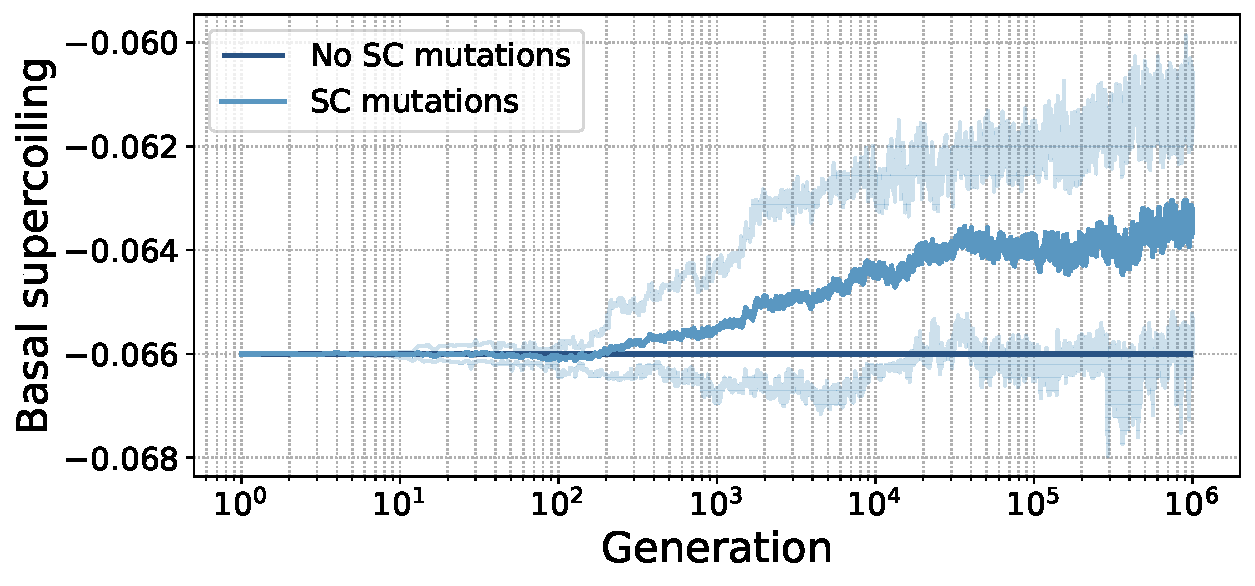
\includegraphics[width=0.75\textwidth]{epistasis/img/basal_sc_all.pdf}
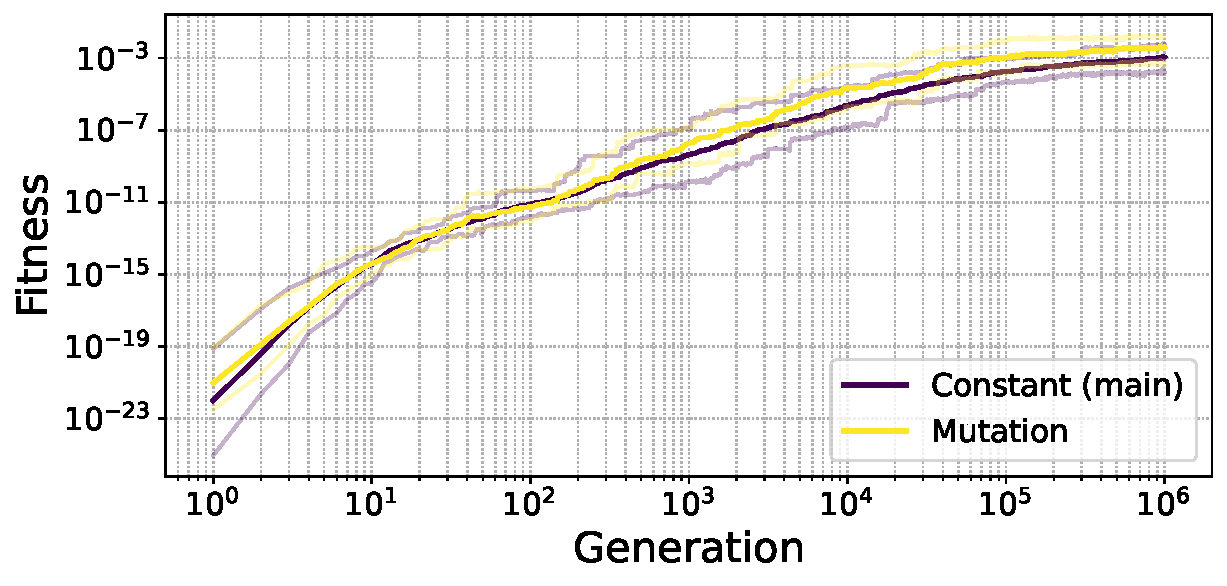
\includegraphics[width=0.75\textwidth]{epistasis/img/fitness_all_with_main.pdf}
\caption[Average basal supercoiling and fitness during evolution of the wild-types, with basal supercoiling level mutations]{Top: average basal supercoiling level of the best individual in every replicate during evolution of the 10 wild-types with (in yellow) and without (in purple) mutations in the basal supercoiling level.
Bottom: average fitness of the best individual in every replicate during evolution, for the wild-types with (yellow) and without (purple) supercoiling mutations.
Lighter lines represent the first and last decile of the data.}
\label{fig:epistasis:wt-evolution}
\end{figure}

Figure~\ref{fig:epistasis:wt-evolution} presents the evolution of the basal supercoiling level (top) and fitness (bottom) of the best individual in each replicate during the evolution of the wild-type populations, with and without supercoiling mutations.
A clear selection pressure towards reducing the amount of negative supercoiling can be observed, as well as a slightly higher fitness throughout evolution of the populations with supercoiling mutations.
A possible hypothesis to explain this higher fitness comes from recalling that, with the initial basal supercoiling level of $\sigma_{basal} = -0.066$, genes tend to have a high expression level, in both environments (see the dash-dotted curve of Figure~\ref{fig:ploscb:activity-by-sigma}).
In that case, decreasing the level of negative supercoiling lessens the bias towards high gene expression in both environments, and therefore helps the inhibition of \emph{A} genes in environment B in these populations (data not shown).

\subsection{Environmental Shock}

\begin{figure}
\centering
\begin{elasticrow}[width=\textwidth]
\elasticfigure{epistasis/img/init_indiv_with-sc00_env_A.pdf}
\elasticfigure{epistasis/img/init_indiv_rep02_env_A.pdf}
\end{elasticrow}
\caption[Evolved wild-type individual before and after an environmental shock]{Genome of one of the control wild-types (left), and shocked individual created from that individual (right), both evaluated in environment A.
Gene types (colors) change, but not the local supercoiling level, as gene positions remain constant.}
\label{fig:epistasis:shock}
\end{figure}

In order to simulate an environmental shock on a given individual, we assign a new type at random to 50\% of the genes of that individual (also chosen at random), ensuring that the number of genes of each type remains constant.
This represents the fact that some genes that had to be activated in the old environment must now be inhibited in the new environment, and vice versa.
A representative example of environmental shock is depicted in Figure~\ref{fig:epistasis:shock}.
On the left-hand side is the genome of an evolved wild-type individual, and on the right-hand side is the result of applying an environmental shock to this individual.
The type (color) of one third of the genes changes, but not the local supercoiling level along the genome, as the gene positions themselves remain unchanged.
As a result, a certain number of genes end up wrongly activated or inhibited, opening the door to compensatory mutations.


\section{Results}

\begin{figure}[H]
\centering
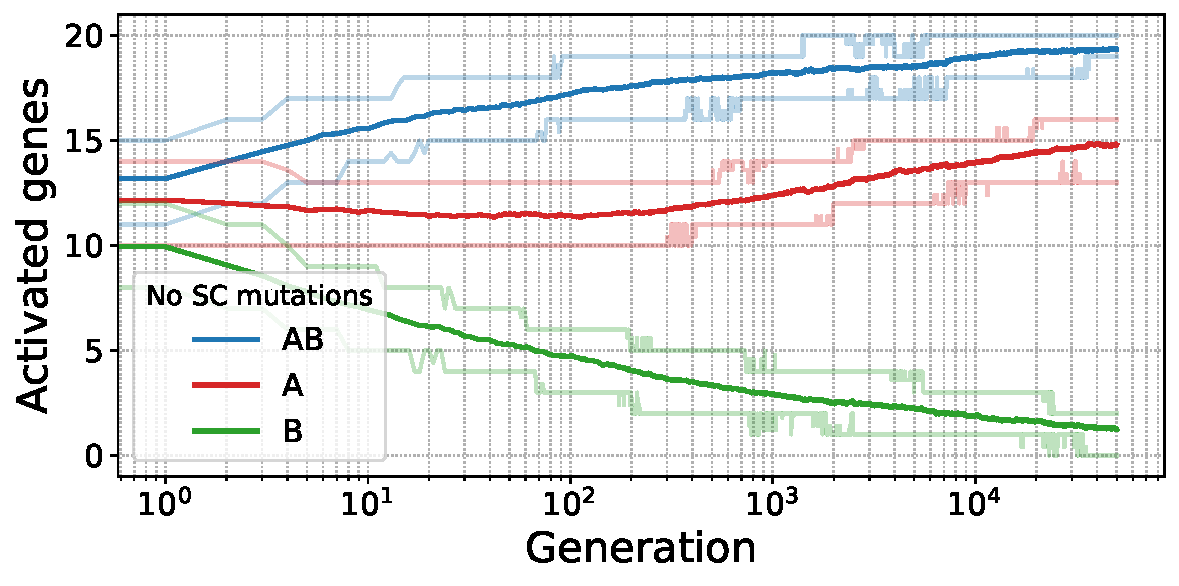
\includegraphics[width=0.495\textwidth]{epistasis/img/control/gene_activity_env_A.pdf}
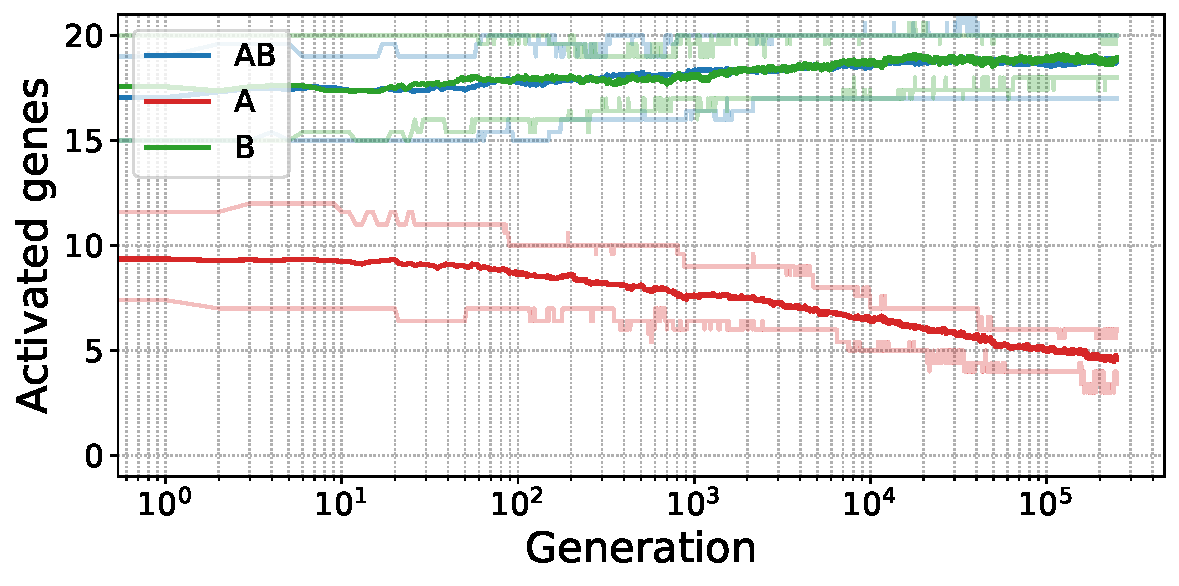
\includegraphics[width=0.495\textwidth]{epistasis/img/control/gene_activity_env_B.pdf}

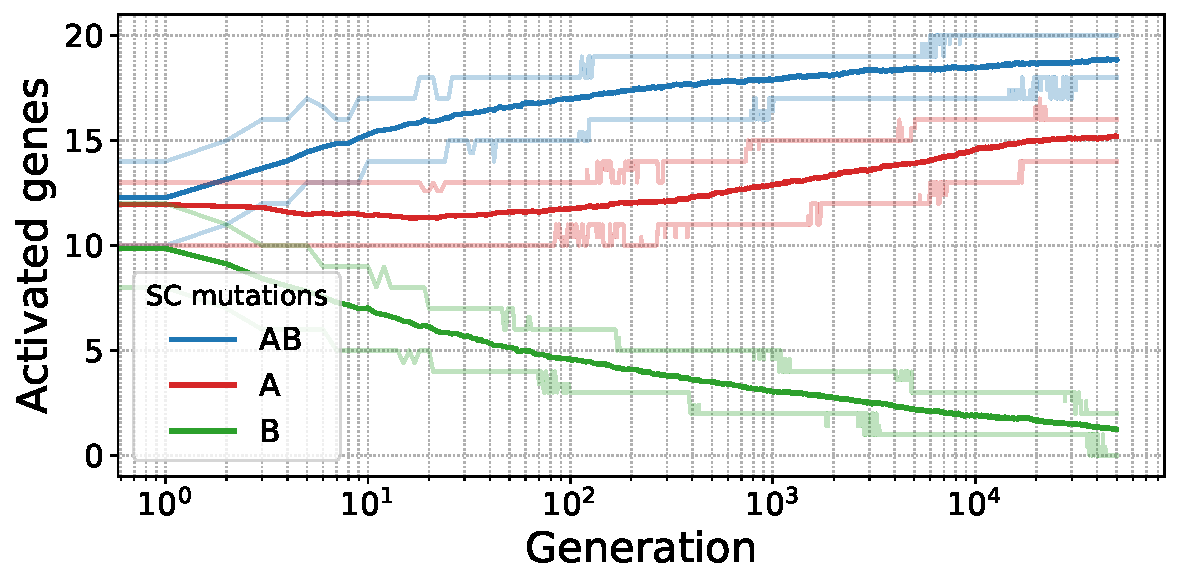
\includegraphics[width=0.495\textwidth]{epistasis/img/with-sc/gene_activity_env_A.pdf}
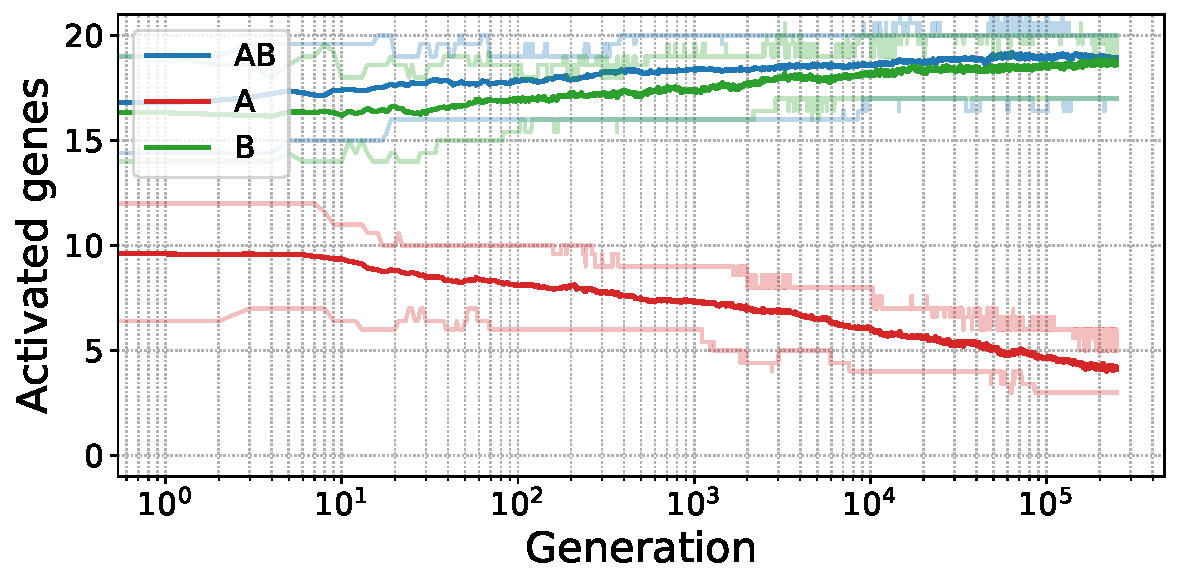
\includegraphics[width=0.495\textwidth]{epistasis/img/with-sc/gene_activity_env_B.pdf}
\caption[Evolution of the number of activated genes in each environment, with a]{Average number of activated genes of each type in environment A (left) and B (right) during evolution, without (top) and with (bottom) supercoiling mutations.}
\label{fig:epistasis:activ-by-env}
\end{figure}

Figure~\ref{fig:epistasis:activ-by-env} shows the evolution of the average number of activated genes by type in each environment after the environmental shocks, averaged over the 25 simulations without supercoiling level mutations (top) and the 25 simulations with supercoiling level mutations (bottom).
In both cases, the number of activated genes in each environment initially regresses towards one half as a consequence of the environmental shock, but evolves again towards their respective targets.

\begin{figure}
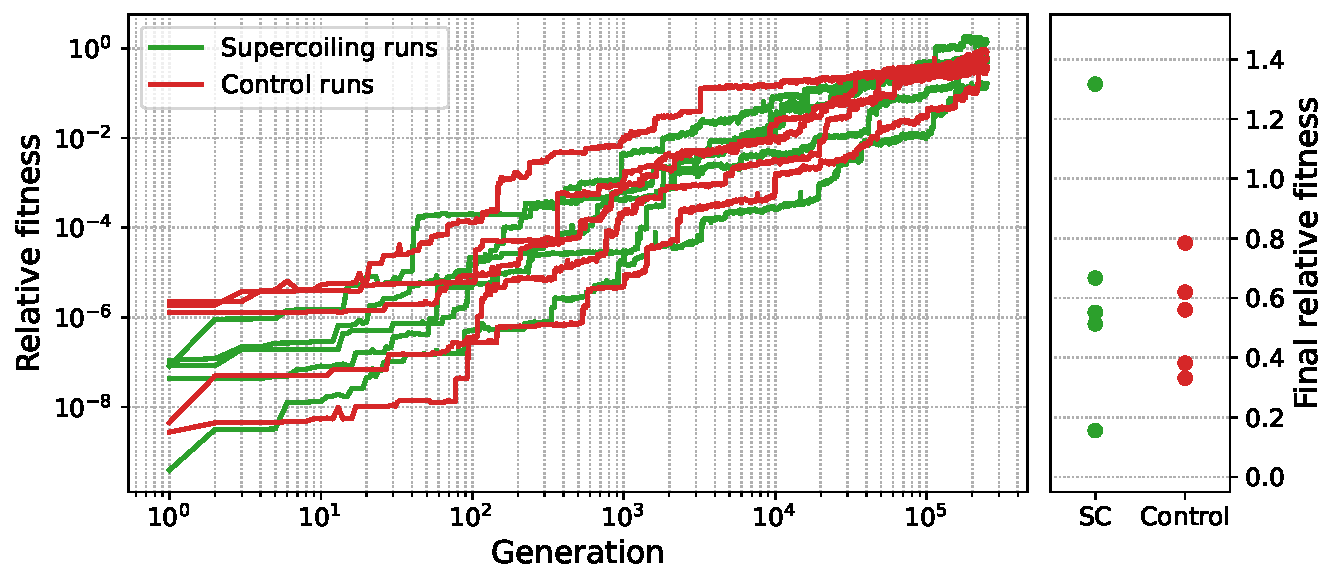
\includegraphics[width=\textwidth]{epistasis/img/rel_fitness_sc_control.pdf}
\caption{Left: relative fitness of the best individual in each simulation compared to the corresponding wild-type, averaged over the 5 replicates for each wild-type, at every generation.
Right: average relative fitness of the 5 replicates for each wild-type at the end of the simulations.}
\label{fig:epistasis:rel-fitness}
\end{figure}

Recall that the point of this experiment is to detect whether populations with supercoiling mutations evolve faster than populations without, which we can interpret as a sign of positive epistasis between supercoiling mutations and other mutations.
In order to be able to compare the speed of evolution between the populations started from the different wild-types, we are therefore interested in the evolution of the fitness of each population compared to its original wild-type.
Figure~\ref{fig:epistasis:rel-fitness} shows the evolution of this relative fitness, averaged over the 5 replicates for each wild-type, both during evolution (left) and at the last generation (right), with (green) or without (red) supercoiling mutations.

Two main observations are possible on the figure.
First, all populations evolve a fitness that is on the same order of magnitude as their ancestor by 250,000 generations, showing that the environmental shock has been successfully compensated during evolution.
Second, we can observe the populations with supercoiling mutations do not seem to evolve faster than the populations without these mutations, as there is no clear separation between the relative fitness curves of each set of populations.
This lack of separation remains in particular true at the last generation of the simulations, as shown on the right-hand side of the figure: the simulations with supercoiling mutations span a broader range of relative fitness values than the simulations without.
These results therefore tend to indicate that, within the context of this experiment, introducing mutations in the basal supercoiling level does not seem to play a role in accelerating evolution, even though it does allow for a higher fitness overall.


\section{Discussion}

In the experiment presented in this chapter, I evaluated the speed at which populations recover their fitness after an environmental shock that changes the expression target of a subset of genes.
I compared the speed of evolution of populations in which the supercoiling basal level evolves and of populations in which it does not, by measuring the relative fitness of each population after 250,000 generations of evolution to their ancestor before the environmental shock.
I was not able to observe a statistically significant difference between the relative fitnesses of each kind of population, which could have been interpreted as a sign of positive epistasis between supercoiling mutations and genomic inversions.

This negative result can be analyzed in several ways.
First, it is of course possible for a signal to appear if I were to increase the number of wild-type individuals subjected to environmental shock, or the number of environmental shocks for each wild-type individual, in order to average out the contingent evolutionary trajectories before and after the shocks.
Given the evolutionary trajectories in Figure~\ref{fig:epistasis:rel-fitness}, this does however not seem very likely.
Second, it is also possible that by analyzing the lineages as in the \emph{Aevol} experiment presented in Chapter~\ref{chap:aevol}, a pattern in which genomic inversions fix faster after a basal supercoiling change could be detected.
Once again, the negative result of the \emph{Aevol} experiment rather diminishes the likeliness of finding such a positive signal.
Finally, the gene expression targets used in the \emph{EvoTSC} model are extremely simple, with the only targets being maximal and minimal expression.
Fitness peaks are therefore separated by extremely wide valleys in the fitness landscape, and basal supercoiling level mutations might not allow population to cross these valleys frequently enough to play a meaningful role in re-adaptation after an environmental shock.
A version of the \emph{EvoTSC} model in which gene expression targets are chosen from a continuous space, rather than a discrete set of values, would not only be more biologically realistic than the current version, but might also present a fitness landscape in which supercoiling mutations can play a more significant evolutionary role.